% IEEEAerospace2012.cls requires the following packages: times, rawfonts, oldfont, geometry
\documentclass[twocolumn,letterpaper]{article}  % only supports two-column, letterpaper format

\usepackage{booktabs}
\usepackage[]{graphicx,latexsym,amssymb,amsfonts,amsmath,amstext,times}
% NOTE: The .cls file is now compatible with amsmath!!!

\usepackage{floatrow}
\usepackage{hyperref}

\newcommand{\ignore}[1]{}  % {} empty inside = %% comment
\usepackage{enumitem}
\setlist[itemize]{leftmargin=*}
\setlist[enumerate]{leftmargin=*}

% Default fixed font does not support bold face
\DeclareFixedFont{\ttb}{T1}{txtt}{bx}{n}{12} % for bold
\DeclareFixedFont{\ttm}{T1}{txtt}{m}{n}{12}  % for normal

% Custom colors
\usepackage{color}
\usepackage{listings}
\usepackage{framed}
\usepackage{caption}
\usepackage{bm}
\captionsetup[lstlisting]{font={small,tt}}

\definecolor{mygreen}{rgb}{0,0.6,0}
\definecolor{mygray}{rgb}{0.5,0.5,0.5}
\definecolor{mymauve}{rgb}{0.58,0,0.82}

\lstset{ %
  backgroundcolor=\color{white},   % choose the background color; you must add \usepackage{color} or \usepackage{xcolor}
  basicstyle=\ttfamily\footnotesize, % the size of the fonts that are used for the code
  breakatwhitespace=false,         % sets if automatic breaks should only happen at whitespace
  breaklines=true,                 % sets automatic line breaking
  captionpos=b,                    % sets the caption-position to bottom
  commentstyle=\color{mygreen},    % comment style
  deletekeywords={...},            % if you want to delete keywords from the given language
  escapeinside={\%*}{*)},          % if you want to add LaTeX within your code
  extendedchars=true,              % lets you use non-ASCII characters; for 8-bits encodings only, does not work with UTF-8
  frame=single,                    % adds a frame around the code
  keepspaces=true,                 % keeps spaces in text, useful for keeping indentation of code (possibly needs columns=flexible)
  columns=flexible,
  keywordstyle=\color{blue},       % keyword style
  language=Python,                 % the language of the code
  morekeywords={*,...},            % if you want to add more keywords to the set
  numbers=none,                    % where to put the line-numbers; possible values are (none, left, right)
  numbersep=5pt,                   % how far the line-numbers are from the code
  numberstyle=\tiny\color{mygray}, % the style that is used for the line-numbers
  rulecolor=\color{black},         % if not set, the frame-color may be changed on line-breaks within not-black text (e.g. comments (green here))
  showspaces=false,                % show spaces everywhere adding particular underscores; it overrides 'showstringspaces'
  showstringspaces=false,          % underline spaces within strings only
  showtabs=false,                  % show tabs within strings adding particular underscores
  stepnumber=1,                    % the step between two line-numbers. If it's 1, each line will be numbered
  stringstyle=\color{mymauve},     % string literal style
  tabsize=4,                       % sets default tabsize to 2 spaces
}
\usepackage{epigraph}
\renewcommand{\textflush}{flushepinormal}

\begin{document}

\title{RPG Dice Simulator}
\author{%
John Karasinski\\
karasinski@gmail.com
}
\date{}

\maketitle

\thispagestyle{plain}
\pagestyle{plain}

%%%%%%%%%%%%%%%%%%%%%%%%%%%%%%%%%%%%%%
\section{Introduction}
%%%%%%%%%%%%%%%%%%%%%%%%%%%%%%%%%%%%%%

\epigraph{\small\itshape God's dice always have a lucky roll.}{Sophocles (497/6 --- 406/5 BC)}%
\vspace{-2em}
\epigraph{\small\itshape God does not play dice.}{Albert Einstein (1879 --- 1955)}%
\vspace{-2em}
\epigraph{\small\itshape God not only plays dice, but also sometimes throws them where they cannot be seen.}{Stephen Hawking (1942 --- \hspace{1.5em})}%

God's use of dice may be disputed, but archaeological evidence shows that humans have been using dice for many thousands of years~\cite{history}. Dice are often used to insert randomness into games of chance, which can lead to wonderfully unpredictable situations. Due to the randomness associated with them, dice are also excellent for bringing everyone to the same level. A king and a peasant have the same odds when rolling a die, and the die does not care who is more wealthy, talented, or desperate. While the result of any individual roll of the die may be random and unpredictable, a basic application of statistics can lead us to make more informed decisions about the likelihood of events.

The only assumption going forward is that we are considering perfect dice. Perfect dice have an equal probability of landing on each face. According to standard die notation, die rolls are given in the form AdX. A and X are variables, separated by the letter d, which stands for die or dice~\cite{dice_notation}. A represents the number of dice, and X represents the number of faces on each die. For example, 1d20 represents one twenty-sided die, and 2d10 represents two ten-sided die. A six-sided die (1d6), for example, would then have a $1/6$ probability of resulting in a 1, 2, 3, 4, 5 or 6. Cheap dice purchased for gaming will not have this property, and will instead slightly favor different outcomes.

As we do not want to spend time throwing dice, we will instead use software to simulate the results of their throws. For the purposes of the simulations here, you can pretend that we have purchased \textit{very, very expensive} dice which behave perfectly. The joy of the software used for this project though, is that it is all 100\% open source and free.

The project outline states: ``Create a function that will allow me to specify the number of dice I want to use per roll, the number of faces on each die (assume all dice used in a roll have the same number of faces), whether I will sum the scores of each die or will have a minimum value needed to count as a success per die, and whether I will include botches or not as an outcome for rolls.'' Several additional statistics were requested to describe the nature of the outcome of 1,000 repetitions of various dice rolls.

%%%%%%%%%%%%%%%%%%%%%%%%%%%%%%%%%%%%%%
\section{Simulation Method}
%%%%%%%%%%%%%%%%%%%%%%%%%%%%%%%%%%%%%%

This simulation will make use of Python 3.5.0 and NumPy 1.10.1. The core idea behind the simulation is to generate pseudorandom numbers to simulate the throwing of dice. The rules given in the project outline (summing, botching) can then be applied to deduce the result of the simulated dice throw.

The basic functionality behind the simulation is the \texttt{dice()} function. This function accepts three arguments, \texttt{A}, \texttt{X}, and an optional \texttt{n}, where \texttt{A} and \texttt{X} take on the same meaning as in standard dice notation, and \texttt{n} is the number of times to simulate the throw. Calling \texttt{dice(3, 6, n=2)}, for example, would return \texttt{array([[2, 2, 6], [5, 3, 4]])}. This array has 2 rows of 3 simulated 6-sided dice. The first row (representing the first throw) contains the values 2, 2, and 6, and the second row contains the values 5, 3, and 4.

The \texttt{dice()} function is essentially a helper function, which calls NumPy's random integer function. NumPy uses the Mersenne twister sequence to generate pseudorandom numbers. As these are psuedorandom numbers and not true random numbers, knowing the seed of the algorithm allows you to reproduce the results, and predict future events with 100\% accuracy. For the purposes of this project, however, pseudorandom numbers will function sufficiently.

The primary function for this simulation is the \texttt{throw()} function, which parses user input and gives raw output, plots, and/or statistics about throws. There are three different ways to use this program. The first way to use this is to simply call \texttt{throw('1d6', n=1000)}. This will return the results of 1,000 1d6 dice rolls. The second way to run this is to call something along the lines of \texttt{throw('1d6', n=1000, plot=True)}. This will return a plot of the the outcomes of 1,000 1d6 dice rolls (a flat distribution from 1 to 6). The third way to use this program is to call \texttt{throw('1d6', n=1000, stats=True)}, which will return the value counts of each outcome of the 1,000 1d6 rolls.

A separate function, \texttt{expected()}, was used to enumerate all possible outcomes for each of the 4 primary scenarios we were asked to investigate. Once enumerated, the exact probability of each outcome was calculated. These exact probabilities were used along with $\chi^2$ tests to statistically confirm that the values from my simulation are the same.

%%%%%%%%%%%%%%%%%%%%%%%%%%%%%%%%%%%%%%
\section{Results}
%%%%%%%%%%%%%%%%%%%%%%%%%%%%%%%%%%%%%%
The script for this project, \texttt{dice.py}, accomplishes all of the scenarios set out in the project outline. The first four scenarios,
\begin{enumerate}
\itemsep-.25em
\item ``Roll 1d20 and I just want to know the score.''
\item ``Roll 2d6 and I want to know my summed scores.''
\item ``Roll 4d10 where I need to roll 5s or greater such that each roll of 5 or greater counts as a success.''
\item ``The same scenario as above, but now each 1 rolled detracts from the number of successes.''
\end{enumerate}
\noindent can be accomplished by running the following code:
\begin{lstlisting}
throw('1d6')
# 2
throw('1d20')
# 15
throw('4d10', success_min=5)
# 4
throw('4d10', success_min=5, botching=True)
# 1
\end{lstlisting}

The second set of four scenarios was to plot and table several statistics from various dice roll scenarios. $\chi^2$ tests were used to compare the expected value counts to the observed value counts. These exact probabilities were used along with $\chi^2$ tests to statistically confirm that the values from my simulation are the same at the 5\% level of significance. $H_0$ is that the distribution of our results from simulated dice rolls is equivalent to the distribution of the results from the exact probabilities. $H_1$ is simply that $H_0$ is false. The results of each scenario are shown below.

\subsection{Roll 1d6 1,000 times, frequency of each outcome?}
This is a very basic scenario. As we are just rolling a single die, we should expect a flat distribution of all the possible outcomes (1-6). The exact probability of each outcome is $1/6 \approx 16.67\%$. The observed dice rolls showed no statistical difference from the exact probability distribution $[\chi^2 (1,N=1000)=6.60, p=0.25]$.

The command to run this scenario is:
\begin{lstlisting}
throw('1d6', n=1000, plot=True, stats=True)
\end{lstlisting}
\begin{figure}[H]
\centering
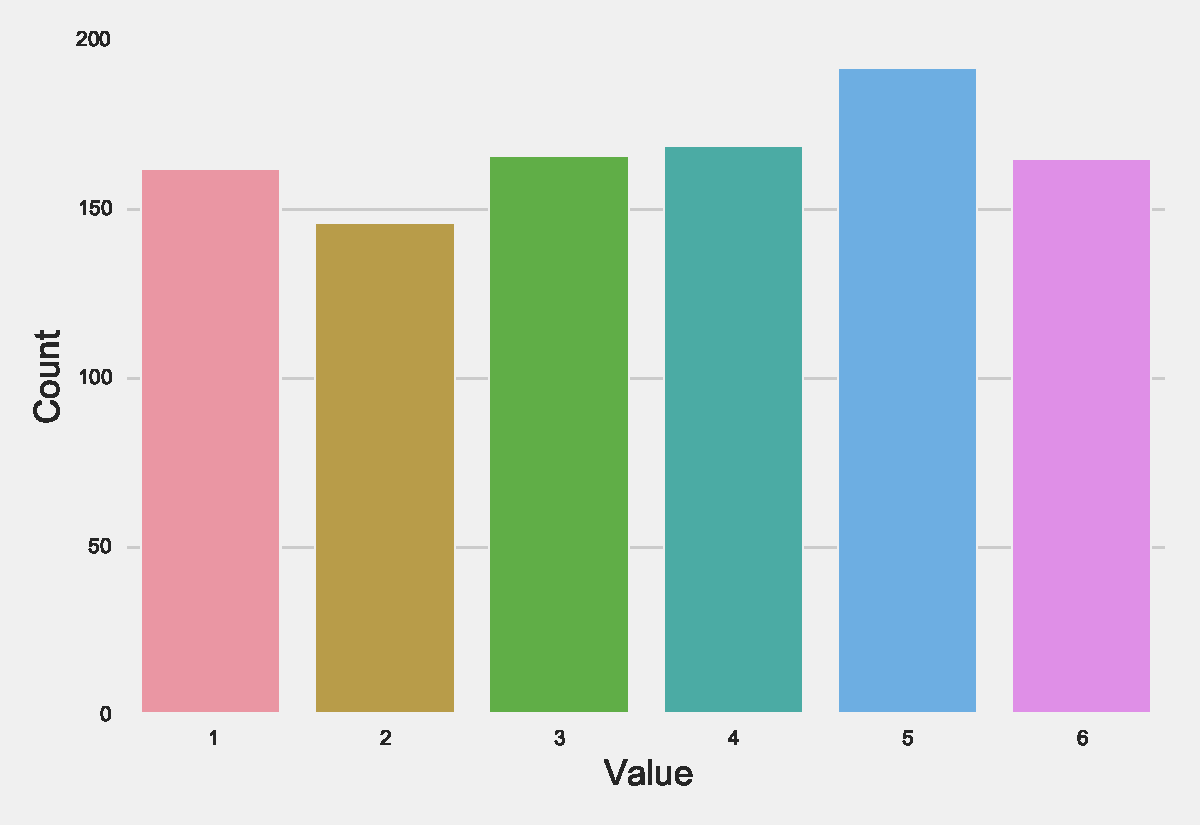
\includegraphics[width=3.25in]{1d6.pdf}
\caption{Results from 1,000 1d6 rolls.}
% \label{fig:on}
\end{figure}

\begin{table}[H]
\begin{center}
\begin{tabular}{*{3}{r}}
\toprule
Value & Count & Frequency \\
\midrule
     1 &   162 &      16.2 \\
     2 &   146 &      14.6 \\
     3 &   166 &      16.6 \\
     4 &   169 &      16.9 \\
     5 &   192 &      19.2 \\
     6 &   165 &      16.5 \\
\bottomrule
\end{tabular}
\end{center}
\caption{Results of 1,000 1d6 rolls}
\end{table}

\subsection{Roll 2d6 1,000 times, frequency of each outcome? Use the summed scores of each die as your outcome.}
This is a slightly more interesting scenario. As we are rolling a two die, we should expect a triangle distribution centered around the most likely combination, 7, and ranging all the possible values (2-12). We can calculate each possible outcome and the probability of each. The observed dice rolls showed no statistical difference from the exact probability distribution $[\chi^2 (1,N=1000)=14.31, p=0.16]$.

This is indeed what we see, with some minor variation due to the low \texttt{n}. The command to run this scenario is:

\begin{lstlisting}
throw('2d6', n=1000, plot=True, stats=True)
\end{lstlisting}

\begin{figure}[H]
\centering
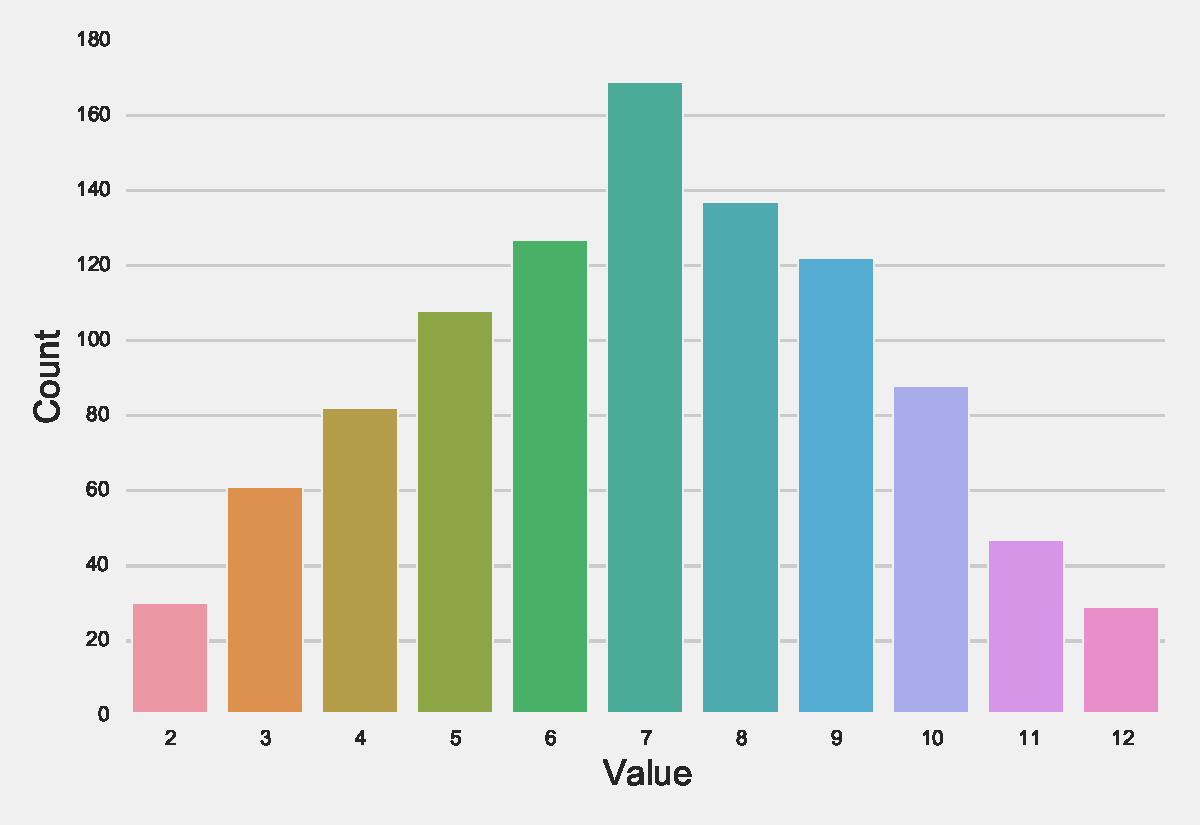
\includegraphics[width=3.25in]{2d6.pdf}
\caption{Results of summed values from 1,000 2d6 rolls.}
% \label{fig:on}
\end{figure}

\begin{table}[H]
\begin{center}
\begin{tabular}{*{3}{r}}
\toprule
Value & Count & Frequency \\
\midrule
     2 &    28 &       2.8 \\
     3 &    57 &       5.7 \\
     4 &    94 &       9.4 \\
     5 &   123 &      12.3 \\
     6 &   139 &      13.9 \\
     7 &   153 &      15.3 \\
     8 &   107 &      10.7 \\
     9 &   129 &      12.9 \\
    10 &    88 &       8.8 \\
    11 &    54 &       5.4 \\
    12 &    28 &       2.8 \\
\bottomrule
\end{tabular}
\end{center}
\caption{Results of summed values from 1,000 2d6 rolls.}
\end{table}

\subsection{Roll 6d10 1,000 times, frequency of each outcome? Treat a score of 6 or better as a success and scores less than 6 as nothing, the outcome is total number of successes (include the frequency of no successes).}

Now we no longer care about the exact outcome of each die, we only care whether or not it is greater than or equal to 6. For a 10 sided die, exactly half of the possible outcomes are counted as successes. We can calculate each possible outcome to generate the exact probabilities. The observed dice rolls showed no statistical difference from the exact probability distribution $[\chi^2 (1,N=1000)=3.26, p=0.78]$.

The following line calculates the statistics for this scenario:
\begin{lstlisting}
throw('6d10', n=1000, success_min=6, plot=True, stats=True)
\end{lstlisting}

\begin{figure}[H]
\centering
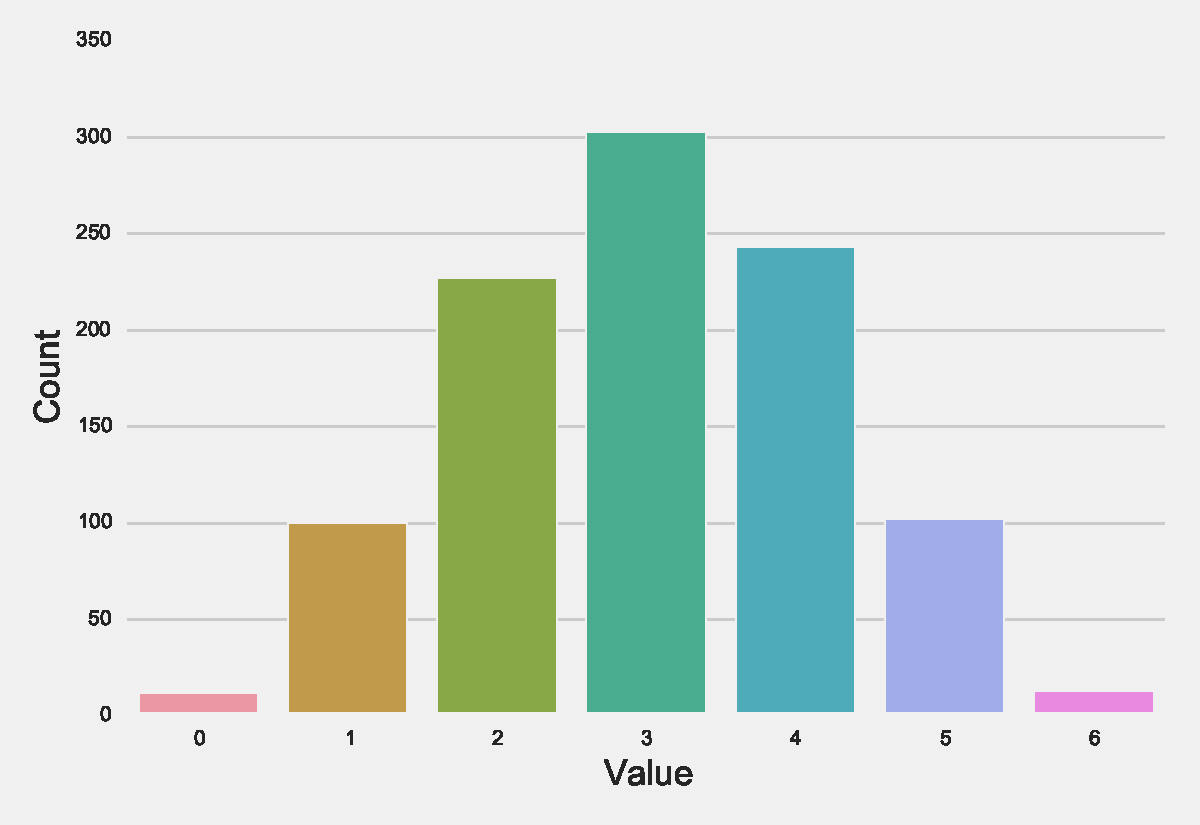
\includegraphics[width=3.25in]{6d10_min6.pdf}
\caption{Results of succeses from 1,000 6d10 rolls, where scores of 6 or greater are considered successes.}
% \label{fig:on}
\end{figure}

\begin{table}[H]
\begin{center}
\begin{tabular}{*{3}{r}}
\toprule
Value & Count & Frequency \\
\midrule
     0 &    12 &       1.2 \\
     1 &   100 &      10.0 \\
     2 &   227 &      22.7 \\
     3 &   303 &      30.3 \\
     4 &   243 &      24.3 \\
     5 &   102 &      10.2 \\
     6 &    13 &       1.3 \\
\bottomrule
\end{tabular}
\end{center}
\caption{Results of successes from 1,000 6d10 rolls, where scores of 6 or greater are considered successes.}
\end{table}

\subsection{Same as (c) above except now scores of 1 count as a botch. Each botch is subtracted from each success. If there are more botches than success (i.e., -1 successes) then the overall outcome is a botch. Now depict the frequency of botching, and total number of successes (as before, include the frequency of no successes).}

This final scenario is very similar to the previous one. For our 10 sided die, there is now a $1/10$ probability of a botch, a $2/5$ probability of a failure, and a $1/2$ probability of a success. We can calculate each possible outcome to generate the exact probabilities. The observed dice rolls showed no statistical difference from the exact probability distribution $[\chi^2 (1,N=1000)=3.64, p=0.82]$.

\begin{lstlisting}
throw('6d6', n=1000, success_min=6, botching=True, plot=True, stats=True)
\end{lstlisting}
\begin{figure}[H]
\centering
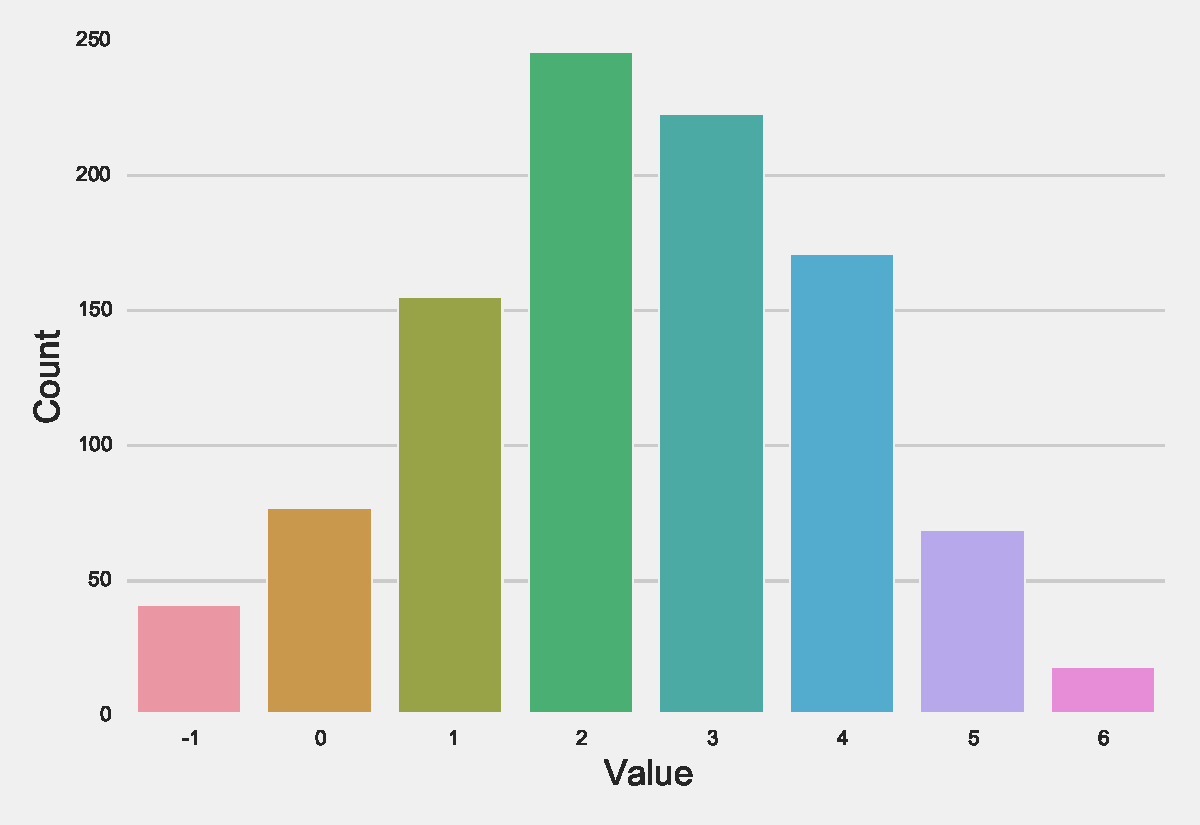
\includegraphics[width=3.25in]{6d10_min6_botching.pdf}
\caption{Results of successes from 1,000 6d10 rolls, where scores of 6 or greater are considered successes, and scores of 1 are considered botches.}
% \label{fig:on}
\end{figure}

\begin{table}[H]
\begin{center}
\begin{tabular}{*{3}{r}}
\toprule
Value & Count & Frequency \\
\midrule
    -1 &    41 &       4.1 \\
     0 &    77 &       7.7 \\
     1 &   155 &      15.5 \\
     2 &   246 &      24.6 \\
     3 &   223 &      22.3 \\
     4 &   171 &      17.1 \\
     5 &    69 &       6.9 \\
     6 &    18 &       1.8 \\
\bottomrule
\end{tabular}
\end{center}
\caption{Results of succeses from 1,000 6d10 rolls, where scores of 6 or greater are considered successes, and scores of 1 are considered botches.}
\end{table}

%%%%%%%%%%%%%%%%%%%%%%%%%%%%%%%%%%%%%%
\section{Summary}
%%%%%%%%%%%%%%%%%%%%%%%%%%%%%%%%%%%%%%


\bibliographystyle{IEEEtran}
%\bibliography{IEEEabr,MyBle}
\begin{thebibliography}{1}

\bibitem{history}
Carlisle, Rodney P., ed. Encyclopedia of play in today's society. Vol. 1. Sage, 2009.

\bibitem{dice_notation}
``Standard Dice Notation''. dice-play. 2006-04-06. Archived from the original on 2007-04-26. https://web.archive.org/web/20070426013749/http://homepage.ntlworld.com/dice-play/Notation.htm

\end{thebibliography}

\clearpage
\onecolumn
%%%%%%%%%%%%%%%%%%%%%%%%%%%%%%%%%%%%%%%%%%%%%%%%%%%%%%%%%%%%%%%%%%%%%%%%%%%%%%%%%%%%%%%%%%%%%%%%%
\appendix{}               % note there is no {} to put a title. Each appendix has its own title
%%%%%%%%%%%%%%%%%%%%%%%%%%%%%%%%%%%%%%%%%%%%%%%%%%%%%%%%%%%%%%%%%%%%%%%%%%%%%%%%%%%%%%%%%%%%%%%%%
% For a single appendix, use the \appendix{} keyword and do not use the \section command.

\section{Source Code}        % first appendix
\lstinputlisting{"../Option 1 Computation/dice.py"}
% %%%%%%%%%%%%%%%%%%%%%%%%%%
% This is the first appendix.

% \subsection{Comments}
% If you have only one appendix, use the ``appendix'' keyword.

% \subsection{More Comments}
% Use section and subsection keywords as usual.

\end{document}

